% Options for packages loaded elsewhere
\PassOptionsToPackage{unicode}{hyperref}
\PassOptionsToPackage{hyphens}{url}
\PassOptionsToPackage{dvipsnames,svgnames,x11names}{xcolor}
%
\documentclass[runningheads
]{llncs}

\usepackage{amsmath,amssymb}
\usepackage{iftex}
\ifPDFTeX
  \usepackage[T1]{fontenc}
  \usepackage[utf8]{inputenc}
  \usepackage{textcomp} % provide euro and other symbols
\else % if luatex or xetex
  \usepackage{unicode-math}
  \defaultfontfeatures{Scale=MatchLowercase}
  \defaultfontfeatures[\rmfamily]{Ligatures=TeX,Scale=1}
\fi
\usepackage{lmodern}
\ifPDFTeX\else  
    % xetex/luatex font selection
\fi
% Use upquote if available, for straight quotes in verbatim environments
\IfFileExists{upquote.sty}{\usepackage{upquote}}{}
\IfFileExists{microtype.sty}{% use microtype if available
  \usepackage[]{microtype}
  \UseMicrotypeSet[protrusion]{basicmath} % disable protrusion for tt fonts
}{}
\makeatletter
\@ifundefined{KOMAClassName}{% if non-KOMA class
  \IfFileExists{parskip.sty}{%
    \usepackage{parskip}
  }{% else
    \setlength{\parindent}{0pt}
    \setlength{\parskip}{6pt plus 2pt minus 1pt}}
}{% if KOMA class
  \KOMAoptions{parskip=half}}
\makeatother
\usepackage{xcolor}
\setlength{\emergencystretch}{3em} % prevent overfull lines
\setcounter{secnumdepth}{-\maxdimen} % remove section numbering
% Make \paragraph and \subparagraph free-standing
\ifx\paragraph\undefined\else
  \let\oldparagraph\paragraph
  \renewcommand{\paragraph}[1]{\oldparagraph{#1}\mbox{}}
\fi
\ifx\subparagraph\undefined\else
  \let\oldsubparagraph\subparagraph
  \renewcommand{\subparagraph}[1]{\oldsubparagraph{#1}\mbox{}}
\fi


\providecommand{\tightlist}{%
  \setlength{\itemsep}{0pt}\setlength{\parskip}{0pt}}\usepackage{longtable,booktabs,array}
\usepackage{calc} % for calculating minipage widths
% Correct order of tables after \paragraph or \subparagraph
\usepackage{etoolbox}
\makeatletter
\patchcmd\longtable{\par}{\if@noskipsec\mbox{}\fi\par}{}{}
\makeatother
% Allow footnotes in longtable head/foot
\IfFileExists{footnotehyper.sty}{\usepackage{footnotehyper}}{\usepackage{footnote}}
\makesavenoteenv{longtable}
\usepackage{graphicx}
\makeatletter
\def\maxwidth{\ifdim\Gin@nat@width>\linewidth\linewidth\else\Gin@nat@width\fi}
\def\maxheight{\ifdim\Gin@nat@height>\textheight\textheight\else\Gin@nat@height\fi}
\makeatother
% Scale images if necessary, so that they will not overflow the page
% margins by default, and it is still possible to overwrite the defaults
% using explicit options in \includegraphics[width, height, ...]{}
\setkeys{Gin}{width=\maxwidth,height=\maxheight,keepaspectratio}
% Set default figure placement to htbp
\makeatletter
\def\fps@figure{htbp}
\makeatother

\usepackage{graphicx,hyperref}
\renewcommand\UrlFont{\color{blue}\rmfamily}
\usepackage[dvipsnames]{xcolor} % colors
\newcommand{\tw}[1]{{\textcolor{blue}{#1}}}
\newcommand{\svp}[1]{{\textcolor{RedOrange}{#1}}}
\newcommand{\eb}[1]{{\textcolor{Green}{#1}}}
\usepackage[capitalise]{cleveref}
\makeatletter
\makeatother
\makeatletter
\makeatother
\makeatletter
\@ifpackageloaded{caption}{}{\usepackage{caption}}
\AtBeginDocument{%
\ifdefined\contentsname
  \renewcommand*\contentsname{Table of contents}
\else
  \newcommand\contentsname{Table of contents}
\fi
\ifdefined\listfigurename
  \renewcommand*\listfigurename{List of Figures}
\else
  \newcommand\listfigurename{List of Figures}
\fi
\ifdefined\listtablename
  \renewcommand*\listtablename{List of Tables}
\else
  \newcommand\listtablename{List of Tables}
\fi
\ifdefined\figurename
  \renewcommand*\figurename{Figure}
\else
  \newcommand\figurename{Figure}
\fi
\ifdefined\tablename
  \renewcommand*\tablename{Table}
\else
  \newcommand\tablename{Table}
\fi
}
\@ifpackageloaded{float}{}{\usepackage{float}}
\floatstyle{ruled}
\@ifundefined{c@chapter}{\newfloat{codelisting}{h}{lop}}{\newfloat{codelisting}{h}{lop}[chapter]}
\floatname{codelisting}{Listing}
\newcommand*\listoflistings{\listof{codelisting}{List of Listings}}
\makeatother
\makeatletter
\@ifpackageloaded{caption}{}{\usepackage{caption}}
\@ifpackageloaded{subcaption}{}{\usepackage{subcaption}}
\makeatother
\makeatletter
\@ifpackageloaded{tcolorbox}{}{\usepackage[skins,breakable]{tcolorbox}}
\makeatother
\makeatletter
\@ifundefined{shadecolor}{\definecolor{shadecolor}{rgb}{.97, .97, .97}}
\makeatother
\makeatletter
\makeatother
\makeatletter
\makeatother
\ifLuaTeX
  \usepackage{selnolig}  % disable illegal ligatures
\fi
\usepackage[]{biblatex}
\addbibresource{refs.bib}
\IfFileExists{bookmark.sty}{\usepackage{bookmark}}{\usepackage{hyperref}}
\IfFileExists{xurl.sty}{\usepackage{xurl}}{} % add URL line breaks if available
\urlstyle{same} % disable monospaced font for URLs
\hypersetup{
  pdftitle={Escaping Flatland: Graphics, Dimensionality, and Human Perception},
  pdfauthor={Susan Vanderplas; Erin Blankenship; Tyler Wiederich},
  pdfkeywords={teaching, graphics, user-study, perception, accuracy},
  colorlinks=true,
  linkcolor={blue},
  filecolor={Maroon},
  citecolor={Blue},
  urlcolor={Blue},
  pdfcreator={LaTeX via pandoc}}

\title{Escaping Flatland: Graphics, Dimensionality, and Human
Perception}
 %title

\author{%
Susan Vanderplas\orcidID{0000-0002-3803-0972}  \and Erin
Blankenship\orcidID{0000-0002-9132-6932}  \and Tyler
Wiederich\orcidID{0009-0006-8131-5822} %
} % author

% First names are abbreviated in the running head.
% If there are more than two authors, 'et al.' is used.
%


\date{}

% \institute{
%   Princeton University, Princeton NJ 08544, USA \and
%   Springer Heidelberg, Tiergartenstr. 17, 69121 Heidelberg, Germany
%   \email{lncs@springer.com}\\
%   \url{http://www.springer.com/gp/computer-science/lncs} \and
%   ABC Institute, Rupert-Karls-University Heidelberg, Heidelberg, Germany\\
%   \email{\{abc,lncs\}@uni-heidelberg.de}
% }
\institute{Statistics Department, University of Nebraska Lincoln\\340
Hardin Hall North Wing, 3310 Holdrege St., Lincoln, NE, USA,
68503 \email{susan.vanderplas@unl.edu}}


\begin{document}
\maketitle
\begin{abstract}
Almost 40 years ago, Cleveland and McGill published the first of 3
papers detailing experiments assessing the accuracy of numerical
perception using different types of charts. This study is often cited as
a reason to avoid the use of extraneous dimensions in data
visualization: 2D bar charts produced more accurate estimates than 3D
bar charts; in addition, lines (length) produced more accurate estimates
than circles (area). Graphics have changed fairly significantly in the
last 40 years: where we once had fixed 3D perspective charts, we now can
rotate 3D renderings in digital space and even 3D print our charts to
examine physically. Many optical illusions result from perceptual
mismatches of 3D visual heuristics and 2D, planar, data representations;
more realistic renderings available with modern tools might change the
outcome of Cleveland and McGill's experimental comparison of 2D vs.~3D
accuracy. In this paper, we present several experiments which replicate
the bar chart portion of Cleveland and McGill's original study,
comparing 2D, 3D fixed perspective, 3D rendered, and 3D printed charts.
We discuss the findings and the importance of replicating classic
experiments using modern technology, as well as the benefits of
incorporating hands-on research in introductory classes as experiential
learning activities.
  \keywords{ teaching  \and  graphics  \and  user-study  \and  perception  \and  accuracy }
\end{abstract}
\ifdefined\Shaded\renewenvironment{Shaded}{\begin{tcolorbox}[frame hidden, boxrule=0pt, sharp corners, enhanced, breakable, borderline west={3pt}{0pt}{shadecolor}, interior hidden]}{\end{tcolorbox}}\fi

Almost 40 years ago, Cleveland \& McGill published the first of 3 papers
detailing experiments assessing the accuracy of numerical perception
using different types of charts. This study is often used to justify
aesthetic advice
\autocite{tufteVisualDisplayQuantitative2001,wainerHowDisplayData1984,kosslynGraphicsHumanInformation1985,kosslynGraphDesignEye2006,wainerPicturingUncertainWorld2009}
to avoid extraneous dimensions in data visualization, though it never
reports experimental results for 3D comparisons.
\textcite{clevelandGraphicalPerceptionTheory1984} create a hierarchy of
elementary perceptual tasks, claiming that 2D bars should be more
accurately perceived than 3D bars; in addition, lines (length) produced
more accurate estimates than circles (area). To support these claims,
they ran a series of experiments described over multiple papers
\autocite{clevelandGraphicalPerceptionTheory1984,clevelandGraphicalPerceptionGraphical1985,clevelandGraphicalPerceptionVisual1987}
assessing the accuracy of participant estimations when making
comparisons between elements of different types of charts. While
estimation precision is not (and should not be) the only goal in
statistical graphics \autocite{bertiniWhyShouldnAll2020}, the advice to
avoid 3D charts persists, even though the charts tested in
\textcite{clevelandGraphicalPerceptionTheory1984} are an extremely
limited version of the different types of 3D charts which we can
generate today.

\hypertarget{technological-innovation}{%
\subsection{Technological Innovation}\label{technological-innovation}}

While 3D computer graphics have existed since Sketchpad was created in
1963 \autocite{sutherlandSketchpadManmachineGraphical1963}, and home
computer software has existed since 1978
\autocite{miyazawa3DARTGRAPHICS1978}, there were significant
developments in 3D software in the 1980s (AutoCAD)
\autocite{walkerAutodeskFile2017}. In the 1990s, 3D charts were
introduced in MS Excel 3.0
\autocite{walkenbachVersionsExcelExplained2021}, and though this might
not be considered an overall improvement, it certainly represented an
innovation in the graphical rendering features available to the average
user. What is undeniable, however, is that since the 1990s, the pace of
3D graphics rendering software (and the hardware to support
ever-increasing detail) has only accelerated. Two important (and
related) software innovations worth mentioning for statistical graphics
are the development of OpenGL \autocite{buss3DComputerGraphics2003},
which is still used in packages such as \texttt{rgl} \autocite{rgl} and
\texttt{moderngl} \autocite{dombiModernGL2024} and WebGL, which made
these graphics available for publication in web browsers
\autocite{parisiWebGLRunning2012,deitsMeshcatdevMeshcatpython2024}.

While Cleveland \& McGill did directly examine volume comparisons in any
of their experiments
\autocite{clevelandGraphicalPerceptionTheory1984,clevelandGraphicalPerceptionGraphical1985,clevelandGraphicalPerceptionVisual1987},
it seems reasonable to conclude that the capabilities to create and
interact with rendered 3D graphics have moved well beyond the simple
image shown in Figure~\ref{fig-vol-chart}; even the full realism of
modern interactive 3D representations is not possible to show in PDF
form; a screenshot of one such chart is shown in
Figure~\ref{fig-modern3d}.

\begin{figure}

\begin{minipage}[t]{0.48\linewidth}

{\centering 

\raisebox{-\height}{

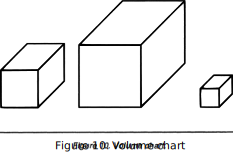
\includegraphics{image/CM1984Fig10_inkscape.png}

}

}

\subcaption{\label{fig-vol-chart}Volume chart recreated from
\textcite{clevelandGraphicalPerceptionTheory1984}. Stimuli used in the
experiment were printed and provided to participants on paper.}
\end{minipage}%
%
\begin{minipage}[t]{0.05\linewidth}

{\centering 

~

}

\end{minipage}%
%
\begin{minipage}[t]{0.48\linewidth}

{\centering 

\raisebox{-\height}{

\includegraphics{image/RenderedChart.png}

}

}

\subcaption{\label{fig-modern3d}Screenshot of a WebGL rendered 3D bar
chart. The WebGL context allows this chart to be manipulated by the
user; rendered shadows, lighting, and other effects contribute to the
realism of the 3D effect.}
\end{minipage}%

\caption{\label{fig-graphical-advances}A comparison of 3D data
renderings from 1984 and 2024.}

\end{figure}

Moreover, we now have the capability to easily create physical objects
from digital renderings using 3D printers. While 3D printing is
typically not fast enough to be used for exploratory data analysis (the
chart in Figure~\ref{fig-modern3d} takes 5 hours to print even at
relatively low quality), it does provide a few advantages over digital
renderings: tactile experience, accessibility for those with visual
impairments, and (for the moment) novelty. More importantly, if we are
interested in comparing realistic 3D renderings to the 3D renderings in
\textcite{clevelandGraphicalPerceptionTheory1984} (or 3D perspective
charts more generally), it is useful to assess both the physical objects
and the digitally rendered images when comparing to the fixed
perspectives used in Figure~\ref{fig-vol-chart}.

\hypertarget{perception-of-graphics}{%
\subsection{Perception of Graphics}\label{perception-of-graphics}}

Because the visual context of 3D graphical renderings has changed so
significantly in the past 40 years, it is important to reassess the
common guidance to avoid using the third dimension in data visualization
in light of new technological capabilities. It is common for artists to
intentionally leverage our 3D visual system to create illusions in two
dimensions that give a three-dimensional effect, as in
Figure~\ref{fig-sidewalk-art}; unfortunately, similar misperceptions can
be unintentionally triggered by common charts: stream graphs,
candlestick charts, and even confidence interval bands.

\begin{figure}

\begin{minipage}[t]{0.48\linewidth}

{\centering 

\raisebox{-\height}{

\includegraphics{image/7006199932_7302488470_o.jpg}

}

}

\subcaption{\label{fig-sidewalk-art}Sidewalk art by Zebit in Liverpool
which leverages visual heuristics to provide the illusion of depth.
Image by \href{https://www.flickr.com/photos/billhunt/7006199932}{Bill
Hunt}.}
\end{minipage}%
%
\begin{minipage}[t]{0.05\linewidth}

{\centering 

~

}

\end{minipage}%
%
\begin{minipage}[t]{0.48\linewidth}

{\centering 

\raisebox{-\height}{

\includegraphics{index_files/figure-pdf/sine-illusion-1.pdf}

}

}

\subcaption{\label{fig-sine-illusion}An illustration of the sine
illusion \autocite{vanderplasSignsSineIllusion2015}, also known as the
line-width illusion. All vertical lines are the same length, but the
lines in the middle of the curve appear to be much shorter.}
\end{minipage}%

\caption{\label{fig-misperception-2d}Two dimensional situations which
create the illusion of three dimensions, either intentionally (a) or
unintentionally (b).}

\end{figure}

A simple example of this phenomenon is shown in
Figure~\ref{fig-sine-illusion}; evenly spaced line segments are shown
following a sine curve; even though each line segment is the same
length, it appears that the segments along the inflection point are much
shorter than the segments at the minimum and maximum of the curve. This
illusion results from misapplied depth perception; the perceived length
of the lines corresponds instead to the width of the line tangent to the
sine curve - that is, the entire series of lines is instead perceived as
a single object that exists in 3 dimensions, and the heuristics which
would normally determine depth are applied to the stimuli, providing an
erroneous estimate of the length of the line. Providing visual stimuli
which are rendered using 3D shading and perspective alleviates the
effects of the sine illusion and allows viewers to estimate line length
properly \autocite[Fig 3]{vanderplasSignsSineIllusion2015}.

It stands to reason, then, that more realistic renderings of
three-dimensional chart objects may alleviate the decreased precision of
quantitative estimates found in
\textcite{clevelandGraphicalPerceptionTheory1984}.

\hypertarget{motivation}{%
\subsection{Motivation}\label{motivation}}

In this paper, we present the results from several experiments designed
to mimic \textcite{clevelandGraphicalPerceptionTheory1984}'s exploration
of different types of grouped bar charts, with the goal of exploring
perception of 2D and 3D charts. We describe the process used to recreate
the stimuli from the original experiment, using 2D, 3D fixed
perspective, 3D rendered, and 3D printed charts to assess estimation
accuracy in a population of undergraduate statistics students. Finally,
we discuss the results of our experiment and the importance of
replicating classic experiments using modern technology. We also
describe the benefits of incorporating hands-on research in introductory
classes as experiential learning activities.

\hypertarget{methodology}{%
\section{Methodology}\label{methodology}}

\hypertarget{participant-recruitment-and-experimental-context}{%
\subsection{Participant Recruitment and Experimental
Context}\label{participant-recruitment-and-experimental-context}}

Participants were recruited from online and in-person sections of
introductory (non-calculus based) statistics courses taught at
University of Nebraska Lincoln during the Summer and Fall of 2023;
overall, students from sections led by 3 different instructors took part
in the experiment. The experiment was integrated into the course as an
experiential learning activity accompanied by several written
reflections. The stages of the experiential learning activity were as
follows:

\begin{enumerate}
\def\labelenumi{\arabic{enumi}.}
\tightlist
\item
  Informed consent - on the LMS during the first 2 weeks of the
  semester.
\item
  Pre-study reflection - on the LMS prior to experiment participation.
  Asks participants to write 3-5 sentences about how scientific
  investigations happen.
\item
  Experiment participation - code from experiment entered into the LMS
\item
  Post experiment reflection - on the LMS after experiment
  participation. Asks participants to guess at the purpose of the
  experiment, what the hypothesis under investigation might have been,
  potential sources of error, what variables were examined, and whether
  they thought there were elements of randomization or experimental
  control.
\item
  Abstract - Students read a 2-page extended abstract written for a
  scientific conference and reflect on how the information presented
  differed from their experience of participating in the experiment.
\item
  Presentation - Students watch a 15-minute conference presentation
  about the experiment and results and reflect on how the information
  presented differed from the information in the abstract.
\end{enumerate}

During step 3, experiment participation, students were provided with an
additional informed consent for the perceptual experiment. Students were
able to opt-out, which prevented their data from being saved, but were
required to at least participate in the process of the experiment to
receive course credit, which ensured that they would be able to reflect
on that experience during the later stages of the experiential learning
activity.

\hypertarget{replicating-cleveland-mcgill}{%
\subsection{Replicating Cleveland \&
McGill}\label{replicating-cleveland-mcgill}}

\begin{figure}

{\centering \includegraphics{image/CM1984Fig4.png}

}

\caption{\label{fig-cm-types}Types of judgments used in
\textcite{clevelandGraphicalPerceptionTheory1984}.}

\end{figure}

We decided to only examine the Type 1 and Type 3 comparisons (e.g.~those
corresponding to grouped bar charts) because multi-color 3D printing was
not supported by equipment we had available, and it was easier to mark
the bars used for comparison if we did not attempt to segment bars
vertically.

Cleveland \& McGill asked participants in the position-length experiment
(described in \autocite{clevelandGraphicalPerceptionTheory1984}) to
evaluate marked bars, first indicating which bar was smaller, and then
estimating ``what percent the smaller is of the larger''. The values
involved in the judgments were
\(s_i = 10 \times 10^{(i-1)/12}, i = 1, ..., 10\), that is,
\(s_i =\{10, 12.12, 14.68, 17.78, 21.54, 26.1, 31.62, 38.31, 46.42, 56.23\}\).
Participants judged ``10 pairs of values with ratios ranging from 0.18
to 0.83''. There are 9 ratios available, as available bar lengths are
equally spaced on the log scale; of these, the study examined 7,
replicating 3 ratios twice, presumably to provide some estimate of
within-participant error. Examining the graphical results in
\textcite{clevelandGraphicalPerceptionTheory1984}, it seems that the
values used were 17.8, 26.1, 38.3, 46.4 (twice), 56.2, 68.1 (twice), and
82.5 (twice). The exact bar lengths corresponding to these ratios were
not disclosed, but we added the additional constraint that no bar length
was used more than twice in the creation of the data sets which would be
rendered in 4 different chart types. Bar heights which were not to be
compared were chosen ``at random, but subject to certain constraints'';
these constraints applied to the stacked bar charts, but not the grouped
bar charts. To mimic this, we used a scaled Beta(2, 2) distribution to
define the size of the other 8 bars not used for comparison.

\hypertarget{experiment-design}{%
\subsection{Experiment Design}\label{experiment-design}}

We created 7 sets of data containing 10 bars lengths, one for each
selected ratio used in
\textcite{clevelandGraphicalPerceptionTheory1984}. These data sets were
assigned colors within chart type (so red in a 3D fixed bar chart
represents a different ratio than red in a 3D printed bar chart),
primarily to facilitate visually checking that combinations of 3D
printed charts in a kit were all of different ratios. Each data set was
rendered in 4 different chart types, with two different bar arrangements
corresponding to Type 1 and Type 3 comparisons. Thus, the experiment
involves \(7 \times 2 \times 4 = 42\) different charts.

Each participant evaluated either 15 or 20 different charts, with a
charts of each display type shown for each of 5 ratios, allocated
according to Figure~\ref{fig-design}. Whether participants were shown
adjacent (Type 1) or separated (Type 2) comparisons was randomly
determined. Participants recruited from online sections of introductory
statistics were shown 2D, 3D fixed, and 3D rendered charts; participants
recruited from in-person sections were shown 2D, 3D rendered, and 3D
printed charts. Due to an application configuration error, some
in-person participants were initially shown 2D, 3D fixed, 3D rendered,
and 3D printed charts, for a total of 20 trials. This error was fixed
after the first 2023 summer session. Figure~\ref{fig-chart-types}
provides example stimuli from each different display type. The order of
trials for each participant was randomly determined by the data
collection app, and in the case of 3D printed chart trials, by the
participant themselves.

In order to facilitate the data collection process, we 3D printed
sufficient charts to create 21 different kits of 5 physical charts each.
Participants in the in-person condition participated in the experiment
during office hours: each participant selected a kit from a bin of
available options and participated in the experiment via the online app
in a quiet study carrel before returning the kit to the bin. The app
asked for a kit ID from in-person participants; this ID was used to
select digital charts which had the same ratios as those in the kit of
3D printed charts. Each day, an instructor would shuffle the kits within
the bin to ensure that each kit had a reasonably equal selection
probability.

\begin{figure}

{\centering \includegraphics{image/design.png}

}

\caption{\label{fig-design}Schematic showing how trials were determined
for each participant.}

\end{figure}

\hypertarget{stimulus-creation}{%
\subsection{Stimulus Creation}\label{stimulus-creation}}

This experiment uses 4 different presentations of grouped bar charts,
shown in Figure~\ref{fig-chart-types}.

\begin{figure}

\begin{minipage}[b]{0.25\linewidth}

{\centering 

\raisebox{-\height}{

\includegraphics{index_files/figure-pdf/2d-bar-1.pdf}

}

\caption{2D}

}

\end{minipage}%
%
\begin{minipage}[b]{0.25\linewidth}

{\centering 

\raisebox{-\height}{

\includegraphics{stimuli/static-3d/static3d-7-1.png}

}

\caption{3D fixed}

}

\end{minipage}%
%
\begin{minipage}[b]{0.25\linewidth}

{\centering 

\raisebox{-\height}{

\includegraphics{image/id04-type1-rep01-rendered.png}

}

\caption{3D rendered}

}

\end{minipage}%
%
\begin{minipage}[b]{0.25\linewidth}

{\centering 

\raisebox{-\height}{

\includegraphics{image/id04-type1-rep01-printed.png}

}

\caption{3D printed}

}

\end{minipage}%

\caption{\label{fig-chart-types}Rendering types used in this experiment.
All charts show the same data.}

\end{figure}

It is relatively simple to create an all-digital experiment and keep
track of the different stimuli (or render them during the experiment
based on the parameters used to create them). With physical stimuli,
this experiment was slightly more complicated, and as a result, we used
slightly different methods to create the 3D files used for both prints
and digital renderings. In particular, we wanted to ensure that each
chart had a label which could not easily fall off or be removed in order
to ensure the ability to audit kit composition reliably. This meant that
the direct plot-to-STL pipeline provided by \texttt{rgl} \autocite{rgl}
and \texttt{rayshader} \autocite{rayshader} was not sufficient. Instead,
we inscribed an ID code (``data/pilot/Set85/id-xx/Typexx-Rep01'') on the
bottom of the base of the charts by creating an OpenSCAD
\autocite{mariuskintelOpenSCADDocumentation2023} template for a grouped
bar chart in OpenSCAD and populated the template with values for each
chart using an R script. The ID code was designed to be informative for
the experimenters but not the participants, as numerical IDs were
randomly assigned to ratio; the use of comparison type in the ID did not
provide any information that would not also be available looking at the
top of the chart.

2D bar charts were created using \texttt{ggplot2} \autocite{ggplot2}
with an extremely minimalist theme. 3D fixed bar charts were created
using Microsoft Excel in order to most accurately represent the angle
used in these sorts of charts `in the wild'. While we could have created
these using some sort of snapshot of the RGL rendering from a fixed
angle, we felt using the same tool used in industry would increase
external validity.

\hypertarget{app-design}{%
\subsection{App Design}\label{app-design}}

Data were collected using a Shiny app \autocite{shiny}. The app first
asked participants for informed consent and basic demographic
information: age range, gender identity, and highest education level,
along with an identifier (``what is your favorite zoo animal'') used as
an additional way to distinguish participants using the applet at the
same time. Participants then were given three practice problems with 2D
charts; these were designed to get participants comfortable with the
online interface and the questions which would be asked, similar to the
way \textcite{clevelandGraphicalPerceptionTheory1984} provided practice
problems (Figure~\ref{fig-practice-screen}) of each type of comparison
in their two experiments.

\begin{figure}

{\centering \includegraphics{image/03-Practice-2.png}

}

\caption{\label{fig-practice-screen}Practice screen providing
participants with guidelines for how to use the sliders and identify the
smaller bar.}

\end{figure}

Just before the experiment started, participants were provided with the
basic trial instructions and asked for a Kit ID (one option was
`online'). Participants who were online were randomly assigned a kit ID
that was used throughout the remainder of the study. During each trial,
participants were asked to evaluate a chart which was either displayed
on the screen or randomly chosen from the kit of physical charts by the
participant (in this case, they were asked to select the chart ID from a
list, as shown in Figure~\ref{fig-chart-id}).

\begin{figure}

{\centering \includegraphics{image/05-Experiment-01-filled-in.png}

}

\caption{\label{fig-chart-id}Screen showing the app process when a 3D
printed chart was randomly selected}

\end{figure}

Participants first identified which bar was smaller, and then used a
slider with no numerical information to show the ratio of the smaller
bar to the larger bar. This differs from the numerical estimation
procedure in \textcite{clevelandGraphicalPerceptionTheory1984}, in that
it does not require participants to estimate the number from the size
ratio, but this difference was intentional - we wanted to reduce
participant cognitive load as much as possible; follow up studies may be
necessary to determine how much of an impact this design decision has on
the results.

At the conclusion of the experiment, participants were provided with a
participation code which could be entered into the learning management
system to receive credit for experiment participation. This code was
provided regardless of whether participants consented to their data
being saved for research purposes.

\hypertarget{results}{%
\section{Results}\label{results}}

\hypertarget{demographics}{%
\subsection{Demographics}\label{demographics}}

Overall, approximately 118 participants met the inclusion criteria
(above the age of majority and a student in the class). This number is
approximate because we recorded data anonymously, and can thus only
track unique sessions where participants completed the demographic
information - this information intentionally cannot be linked to
responses for privacy purposes.

\begin{figure}

\begin{minipage}[t]{0.33\linewidth}

{\centering 

\raisebox{-\height}{

\includegraphics{index_files/figure-pdf/fig-demographics-1.pdf}

}

}

\subcaption{\label{fig-demographics-1}Age}
\end{minipage}%
%
\begin{minipage}[t]{0.33\linewidth}

{\centering 

\raisebox{-\height}{

\includegraphics{index_files/figure-pdf/fig-demographics-2.pdf}

}

}

\subcaption{\label{fig-demographics-2}Gender Identity}
\end{minipage}%
%
\begin{minipage}[t]{0.33\linewidth}

{\centering 

\raisebox{-\height}{

\includegraphics{index_files/figure-pdf/fig-demographics-3.pdf}

}

}

\subcaption{\label{fig-demographics-3}Education}
\end{minipage}%

\caption{\label{fig-demographics}Participant Demographics. As
participants were recruited from undergraduate statistics classes,
imbalances in age, gender, and education level are to be expected.}

\end{figure}

Of these students, there were 100 participants who completed at least 10
trials.

\hypertarget{data-cleaning}{%
\subsection{Data Cleaning}\label{data-cleaning}}

In studies where participants are asked to perform a task, it is
typically important to utilize both attention checks (semi-obvious
answers that check whether the participant is paying attention) and to
be aware of participants who try to submit the study as quickly as
possible without completing the task as directed. In this study, we
asked participants to identify the smaller marked bar, as in the
original study. Of the 1422 trials completed by the 100 participants
with at least 10 trials, 92.28\% identified the correct bar. Trials
where this attention check was not answered correctly have been excluded
from the study with the rationale that the ratio between the smaller and
larger bar (which is limited to a range of 0 - 100\%) is nonsensical if
the smaller bar is not identified correctly.

In addition, we noticed that 15.12\% of the trials completed had a
response of exactly 50\% (the default value of the slider). In
particular, 13 participants completed at least 50\% of trials with a
response of exactly 50\%; these participants have been excluded from the
study on the grounds that they were clearly not engaging with the
purpose of the experiment.

After applying these basic criteria for inclusion in the data analysis,
we have 1276 trials completed by 87 participants remaining for further
analysis.

\hypertarget{summary-statistics}{%
\subsection{Summary Statistics}\label{summary-statistics}}

There are far fewer trials of 3D printed charts, largely because only
online sections were offered during the summer, and relatively few
in-person sections participated in this experiment during the fall
(Figure~\ref{fig-summary}). As a result, we will exclude the 3D printed
charts from further analysis in this study.

\begin{figure}

{\centering \includegraphics{index_files/figure-pdf/fig-summary-1.pdf}

}

\caption{\label{fig-summary}Number of trials across ratio and plot
display type.}

\end{figure}

Examining participant responses in Figure~\ref{fig-violin-accuracy}, it
is clear why \textcite{clevelandGraphicalPerceptionTheory1984} worked
with the midmeans of the responses - there is quite a bit of variability
in the estimates created by participants, sometimes in ways that do not
make much sense.

\begin{figure}

{\centering \includegraphics{index_files/figure-pdf/fig-violin-accuracy-1.pdf}

}

\caption{\label{fig-violin-accuracy}Violin plots of responses relative
to true ratio values. It is clear that some participants misunderstood
the estimation task, while others simply did not move the slider from
50\%. Nonetheless, there is a general relationship between the true
ratio and the central values of the distribution of estimates. Note that
3D printed plots have been removed from this chart because there were
too few responses to estimate a distribution.}

\end{figure}

\hypertarget{midmeans-analysis}{%
\subsection{Midmeans analysis}\label{midmeans-analysis}}

If we repeat the analysis performed in
\textcite{clevelandGraphicalPerceptionTheory1984}, examining a 25\%
trimmed mean of the log absolute error (with a correction),
\[\log_2\left(\left| \text{Estimated Percent} - \text{True Percent}\right| + ^1\!\!/_8\right),\]
we find that there are very few differences across plot types. Comparing
to the actual values reported in Cleveland \& McGill, however, we find
that errors are much higher in this population under the web-based
protocol we are using for data collection than similar midmeans and
intervals reported in \textcite{clevelandGraphicalPerceptionTheory1984}.
Our errors are also larger than those reported in
\textcite{heerCrowdsourcingGraphicalPerception2010}, which used an
online sample but otherwise followed essentially the same procedures
using similar stimuli to
\textcite{clevelandGraphicalPerceptionTheory1984}. It is possible that
introductory statistics students do not estimate as accurately as
academics and their wives
\autocite{clevelandGraphicalPerceptionTheory1984} or paid participants
through Amazon Mechanical Turk
\autocite{heerCrowdsourcingGraphicalPerception2010}; certainly, the
number of participants removed for answering 50\% for all trials
suggests that at least some participants did not take the task
seriously. Another potential explanation is that some of these issues
stem from the measures we took to minimize cognitive load while avoiding
rounding and clustering of responses around benchmark values. In this
study, we used a slider with endpoints marked 0 and 100, but no other
numerical feedback was provided - no tick marks, no value of the current
estimate. While our goal was to remove rounding tendencies, it is
entirely possible that we instead introduced higher error values because
participants could not do the spatial mapping operation without going
through numeric values; then, participants had to invert this process
and map back onto a spatial dimension without any visual aids. Further
studies will be necessary to distinguish between these two issues. It
may also be helpful to provide feedback on a few demo trials before
participating in the experiment in order to ensure that everyone is
comfortable with the input mechanisms; the current demo may not provide
enough active feedback to really get participants familiar with the
interface.

\hypertarget{student-responses}{%
\subsection{Student Responses}\label{student-responses}}

Part of the goal of using this experiment as an experiential learning
activity was to introduce the idea that not all charts are equally
effective to introductory statistics students. In addition, we hoped to
reinforce concepts taught in class, such as randomization, experimental
control, blocking, and interpretation of results, using experiential
learning to help students make the connection between theoretical
concepts and how these concepts play out in real life.

In Fall 2023, this project was offered to students in a 75-person
section of online introductory statistics as extra credit. About 40
students both participated and consented to having their responses
shared across the 6 different parts of the experiment; only 4 of these
components have meaningful responses beyond the question of providing
informed consent or a completion code for the experiment, and of these,
we will briefly consider questions from the post-experiment reflection,
abstract presentation, and presentation. The pre-experiment reflection,
which asked students to think about how scientific experimentation
works, is less specific to this experiment and will thus be omitted.

In the next 3 subsections, we will provide some brief excerpts from
student responses which provide some insight into student learning and
engagement with the experiment. Text files with all student responses
for each question are available on github.

\hypertarget{post-experiment-reflection}{%
\subsubsection{Post-experiment
reflection}\label{post-experiment-reflection}}

Students were asked to complete a reflection activity 1-2 weeks after
completing the experiment, with questions designed to encourage them to
assess how material from the course applied to their experience.

\textbf{What hypotheses might the experimenter have been testing?}

\begin{itemize}
\tightlist
\item
  ``Students will get progressively less accurate as questions were
  asked''
\item
  ``Do students change their answers when asked the same question over
  and over?''
\item
  ``3D printed bar charts will lead to more accurate ratio judgments
  compared to 2D or 3D digital charts.''
\item
  ``That 2d is preferred over 3d. It cleans up the data presentation.''
\item
  ``The public can more accurately understand data when it is provided
  to them in a 2-D graph format.''
\end{itemize}

While some of these hypotheses are not correct (and even amusing), over
half of the students made some mention of the use of different types or
different dimensionality of graph presentations in their answers, and
several more provided reasonable hypotheses about e.g.~the use of
adjacent bars vs.~separated bars in comparisons.

\textbf{What sources of error are involved in this experiment?}

\begin{itemize}
\tightlist
\item
  ``Fatigue effect over the course of making many judgments, learning
  patterns from seeing the same ratios multiple times, possibly
  difference in eyesight among participants.''
\item
  ``There are no line values to help measure it when there is a small
  difference between the graphs.''
\item
  ``People that are guessing''
\item
  ``People in the sample misunderstanding directions.''
\end{itemize}

Here, it is clear that students were capable of identifying many of the
same sources of error that we have identified when considering the large
variability in our results relative to previous studies.

When asked which variables the experimenter examined and whether these
variables were quantitative or categorical, students overwhelmingly
(37/41) indicated at least some understanding of the response variables
(smaller/larger, \% of smaller to larger), and many participants also
identified manipulated variables (chart type) and demographic variables
(age, gender identity, education level) that may have also been of
interest.

\textbf{What elements of experimental design, such as randomization or
the use of a control group, do you think were present in the experiment?
Why?}

\begin{itemize}
\tightlist
\item
  ``I believe every graph was randomized for every student. I also
  believe the practice was meant to be a bit of the control group.''
\item
  ``Randomization was used as participants all received different sets
  of graphs to examine. A person wasn't assigned to a certain set of
  graphs and it was up to random chance on which set of graphs they
  received.''
\item
  ``I think that there is randomization but not a control group in my
  opinion, because there isn't one group that is left alone or not
  studied\ldots.''
\item
  ``Randomization was not used because it was offered as an extra credit
  assignment in class.''
\end{itemize}

These responses indicate that participants were actively considering how
their experience of the experimental design matched terms used in class.
While the final excerpt represents a misunderstanding of the difference
between randomization and random sampling, it is clear from these
comments that students are using their experience and considering the
terms they've learned in class based on those experiences.

\hypertarget{abstract-reflection}{%
\subsubsection{Abstract reflection}\label{abstract-reflection}}

A few weeks after the post-experiment reflection, students were provided
with a 2-page extended abstract that described the experiment in a style
which was consistent with submission to a conference. Students were
asked only a single question, which was \textbf{What components of the
experiment are clearer now than they were as a participant? What
questions do you still have for the experimenter?}

\begin{itemize}
\item
  ``I believed that one of the components was the dimension of the
  graph. However I also thought that the color was the main component
  and that was not true. The angle was an obvious component I felt, but
  then again I wondered if it looked that way because I was using my
  phone.''\footnote{Note that students were explicitly instructed to use
    a laptop (and one was available for their use); it isn't surprising
    that this student had a hard time using a device with a much smaller
    screen.}
\item
  ``The exam was about perceptual judgement, using the difference
  between 2D and 3D graphics. This is a different approach than just
  deciding how much bigger or smaller something is as the participant. A
  question I have is why we think 3D graphs are harder to perceive than
  a 2D graph. This seems a bit confusing to me, because they seem to be
  about the same for me. I also would like to know about the difference
  between 2D rendered charts compared to a 3D printed chart. Perhaps
  this is because I took this course online.''
\item
  ``The scientific question is more clear after reading the extended
  abstract. I now understand that they wanted to compare differences
  between 2-dimension, 3-dimension, and printed 3-dimension. They were
  testing not the correctness, but the perceptual judgment. There was
  also a formula that they provided for judging how the participant
  analyzed the bar graphs, and if they were correct provided the
  formula. The random distribution of ratios also makes sense in that
  there were 21 different combinations of bar graphs amongst different
  participants.''
\item
  ``After reading on the study, I can better understand the reasoning
  behind it and the purpose of the experiment. I enjoyed that they tried
  using similar tactics as that of Cleveland and McGill. I thought it
  was unique that they had strategically planned out the distance
  between the two bars that were being assessed throughout the study, as
  I didn't think it was possible to be that in depth and in such detail.
  Overall, I am impressed by the experiment.''
\item
  ``After reading the abstract, I was surprised to learn that the
  subject of the study wasn't the hypothesis I thought it was. Now it's
  very clear that there's a discrepancy between interpreting 3D and 2D
  graphs/visuals. I am still curious after reading this what the results
  of the study are based on students feedback. I also want to know if
  the student results were different then what was expected based on
  Cleveland/ McGill's study.''
\end{itemize}

Generalizing beyond the excerpts included here, almost all of the
students seemed to enjoy finding out what the experiment was about, and
came up with reasonable and cogent questions about the experiment beyond
what was in the abstract.

\hypertarget{presentation-reflection}{%
\subsubsection{Presentation reflection}\label{presentation-reflection}}

As a final component of this experiment, participants were asked to
watch a 15 minute conference-style presentation of the results and
reflect on the experiment and information present in the abstract
vs.~the presentation.

\textbf{If you had to hear about this study using only the extended
abstract or only the presentation, which one would you prefer? Which one
would be better for determining whether the experiment was well
designed?}

\begin{itemize}
\tightlist
\item
  ``Again I like the presentation better mostly because it adds a more
  personal touch! The abstract is probably really the best was to
  understand the design of the experiment. However I struggle reading
  that kind of material. So for a participant, the video presentation
  was the best.''
\item
  ``I would prefer the presentation. I think that maybe the abstract
  would be better for determining whether the design of the experiment
  was better because of the fact that it strictly lays out the
  experiment and some of what math was involved, whereas even though the
  presentation did that, it went more in depth about the results as well
  instead of just the design.''
\item
  ``I would prefer hearing about the study using the abstract. I believe
  it provides more detail on the setup of the experiment, which is
  better for determining if it was well designed.''
\item
  ``If I had to hear about this study using only one source, I would
  prefer the video presentation. This may be because I am a visual and
  auditory learner, but I also had a hard time understanding what the
  researchers wanted us to get out of the abstract because it was so
  complex. With the presentation, I was able to understand step by step
  how the study was conducted.''
\end{itemize}

While participants were decidedly mixed on their preferred information
transfer method, most agreed that the extended abstract was preferable
for understanding design details, while the presentation was more
engaging.

One goal of the introductory statistics class at UNL is to create
informed consumers of statistical information. As part of that goal, we
asked participants to reflect on what information was available to them
at each stage of this project.

\textbf{How did the information you gained from the components of this
project (participation, post-study reflection, extended abstract,
presentation) differ?}

\begin{itemize}
\tightlist
\item
  ``Participation gathers real-time, subjective feedback. Post-study
  reflection provides deeper insights. The extended abstract offers a
  formal summary, while the presentation conveys findings to a broader
  audience. Each component serves a unique role in understanding
  perceptual judgments on 3D printed bars.''
\item
  ``The experiment itself didn't make it obvious that 2D presentation of
  a graph distorts the data, which is an interesting perspective to
  carry when reading different charts, especially bar graphs. I learned
  this through the extended abstract and presentation, which drastically
  changed my thought process when reflecting on why each type of graph
  led me to believe it had that specific ratio on the slider tool.''
\item
  ``I think that with each module, we gained more and more insight into
  the study and its purpose. It was almost like this video was the last
  part of a scavenger hunt to find the purpose and idea behind the study
  and the other components were like little puzzle pieces.''
\item
  ``As a participant in the study, having no idea what the purpose was
  at first, I truly enjoyed the experiment. I felt like I was doing a
  self-challenge to try and accurately determine how much smaller the
  smaller graph was. Next, I read the extended abstract and appreciated
  the purpose of the experiment, its history behind it, and the
  strategies used within the experiment. When doing the post-study
  reflection, I feel like I got to tie everything together that I had
  learned so far. Finishing off with the presentation, I feel like
  everything became full circle and I found interest in the additional
  information that was given that wasn't in the extended abstract.''
\item
  ``I did not realize the depth of thought that goes into experimental
  design. As a participant, I had no idea of the depth of the research
  for this data. Also as I moved through this process it gave me a
  clearer understanding of the study and its implications. This
  experiment also helped give me experience in understanding the
  experiment design process.''
\end{itemize}

Many participants expressed a feeling that information was gradually
uncovered over time; the sequential unveiling of information seems to
have provided an ongoing engagement and even investment in the study's
results, for those who responded. Interestingly, several participants
mentioned that the post-study reflection was key for their understanding
of the experiment - as no additional information was provided in this
reflection, this suggests that the explicit direction to consider how
concepts learned in class related to the experiment was a useful
exercise for students.

\hypertarget{discussion}{%
\section{Discussion}\label{discussion}}

While this experiment lacked the precision necessary to provide useful
insight into visualization design, the process of incorporating these
experiments into introductory statistics classes seems to be a valuable
tool for motivating student learning. It is possible that we may be able
to reduce response variance in future iterations of this experiment by
providing numerical feedback, strictly numerical estimation methods, or
otherwise manipulating how students interact with the study. One of the
potential explanations for differences between our study and
\textcite{clevelandGraphicalPerceptionTheory1984} is that we used
numerical sliders; however, another explanation is that students did not
estimate ratios with the same amount of care as participants in previous
studies. Certainly, it is possible to read some of the student
reflections and come to the conclusion that some students simply did not
read the instructions or participate in good faith.

A much more valuable outcome of this experiment is that participants
seemed to enjoy the overall process of participation in the study and
reflection upon the experience during the course of their introductory
statistics class. While we did not collect information which allows us
to assess whether participation increased student learning, we can see
from their reflections that most students were able to make connections
between participation in the study and concepts in class when prompted
to think about these topics. Moreover, students seem to enjoy the
``reveal'' moments when reading the abstract and watching the
presentation. The sense of completing a puzzle was evident in many of
the written responses, and it seems likely that the experience of
questioning, forming a hypothesis, and having the hypothesis either
supported or rejected through new information may stick with them after
the concepts in the course are forgotten. In that sense, this experiment
was a success, and embedding basic research and experiential learning in
statistics courses may prove to be a valuable pedagogical tool.


\printbibliography[title=References]


\end{document}
